\def\CTeXPreproc{Created by ctex v0.2.12, don't edit!}\documentclass{beamer}
\usepackage{graphicx}
\usepackage{verbatim}
\usepackage{amsmath}
\usepackage{amsfonts}
\usepackage{setspace}
% \usepackage{beamerthemesplit} // Activate for custom appearance

\title{ANOVA}
\author{Dr. Frank Wood}

\date{}

\DeclareMathOperator*{\Ave}{\mathbb{E}}
\DeclareMathOperator*{\Var}{Var}

\begin{document}

\frame{\titlepage}

\frame[t] {
 \frametitle{ANOVA}
\begin{enumerate}
\item ANOVA is nothing new but is instead a way of organizing the parts of linear regression so as to make easy inference recipes.

\item Will return to ANOVA when discussing multiple regression and other types of linear statistical models.

\end{enumerate}
}

\frame[t] {
 \frametitle{Partitioning Total Sum of Squares}
\begin{enumerate}
\item  ``The ANOVA approach is based on the partitioning of sums of squares and degrees of freedom associated with the response variable
Y''

\item  We start with the observed deviations of $Y_i$ around the observed mean
$$Y_i - \bar{Y}$$
\end{enumerate}
}

\frame[t] {
 \frametitle{Partitioning of Total Deviations}
\begin{figure}
  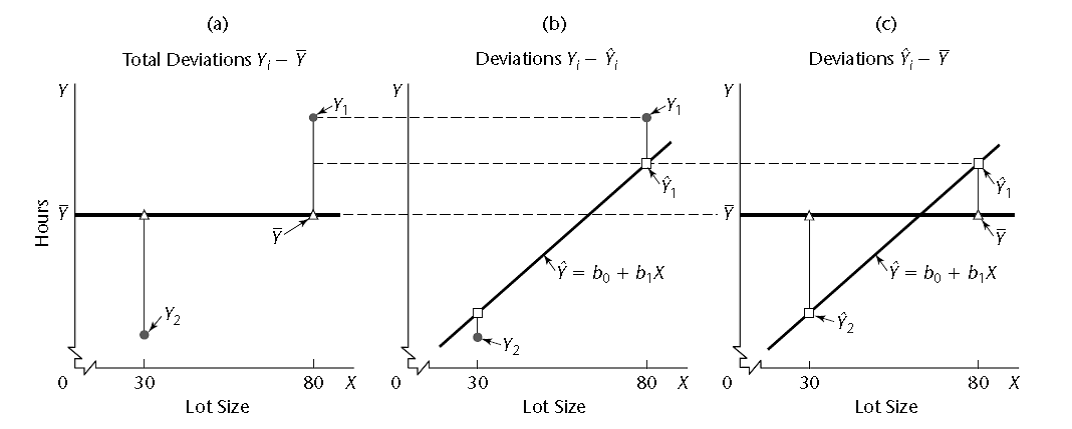
\includegraphics[height=40mm]{partition.png}
\end{figure}
}

\frame[t] {
 \frametitle{Measure of Total Variation}
\begin{enumerate}
\item  The measure of total variation is denoted by $$SSTO = \sum (Y_i - \bar{Y})^2$$
\item  SSTO stands for total sum of squares
\item  If all $Y_i's$ are the same, SSTO = 0
\item  The greater the variation of the $Y_i's$ the greater SSTO
\end{enumerate}
}

\frame[t] {
 \frametitle{Variation after predictor effect}
\begin{enumerate}
\item  The measure of variation of the $Y_i's$ that is still present when the predictor variable X is taken into account is the sum of the squared deviations
$$SSE = \sum (Y_i - \hat{Y_i})^2$$
\item  SSE denotes error sum of squares
\end{enumerate}
}

\frame[t] {
 \frametitle{Regression Sum of Squares}
\begin{enumerate}
\item The difference between SSTO and SSE is SSR
$$SSR = \sum (\hat{Y_i} - \bar Y )^2$$
\item  SSR stands for regression sum of squares
\end{enumerate}
}

\frame[t] { %%% DONT KNOW HOW TO CHANGE LINE IN UNDERBRACE%%%
 \frametitle{Partitioning of Sum of Squares}
$$\underbrace{Y_i - \bar{Y}}_{\text{Total
deviation}} = \underbrace{\hat{Y_i} - \bar{Y}}_{\text{Deviation of
fitted regression value around mean}} +\underbrace{ Y_i -
\hat{Y_i}}_{\text{Deviation around fitted regression line}}$$ }

\frame[t] {
 \frametitle{Remarkable Property}
\begin{enumerate}
\item  The sums of the same deviations squared has the same property!
$$(Y_i - \bar{Y})^2 = (\hat{Y_i} - \bar{Y})^2  + (Y_i - \hat{Y_i})^2$$or $SSTO = SSR +
SSE$
\item Proof:
\end{enumerate}
}

\frame[t] {
 \frametitle{Remarkable Property}
Proof: $(Y_i - \bar{Y})^2 = (\hat{Y_i} - \bar{Y})^2  + (Y_i -
\hat{Y_i})^2$
\begin{eqnarray*}
(Y_i - \bar{Y})^2 &=& \sum[(\hat{Y_i} - \bar{Y})  + (Y_i - \hat{Y_i})]^2 \\
&=& \sum[(\hat{Y_i} - \bar{Y})^2  + (Y_i - \hat{Y_i})^2 +2 (\hat{Y_i} - \bar{Y})(Y_i - \hat{Y_i})] \\
&=& \sum(\hat{Y_i} - \bar{Y})^2  + \sum (Y_i - \hat{Y_i})^2 +2 \sum
(\hat{Y_i} - \bar{Y})(Y_i - \hat{Y_i})
\end{eqnarray*}
but $$\sum (\hat{Y_i} - \bar{Y})(Y_i - \hat{Y_i} ) =  \sum\hat{Y_i}
(Y_i - \hat{Y_i} ) -  \sum \bar{Y} (Y_i - \hat{Y_i} ) =0$$ By
properties previously demonstrated }

\frame[t] {
 \frametitle{Remember: Lecture 3}
\begin{enumerate}
\item  The $i^{th}$ residual is defined to be $$e_i = Y_i - \hat Y_i$$
\item  The sum of the residuals is zero:
\begin{eqnarray*}
\sum_i e_i &=& \sum(Y_i -b_0 -b_1 X_i) \\
&=& \sum Y_i - n b_0 - b_1 \sum X_i \\
&=& 0
\end{eqnarray*}
By first normal equation.
\end{enumerate}
}

\frame[t] {
 \frametitle{Remember: Lecture 3}
The sum of the weighted residuals is zero when the residual in the
$i^{th}$ trial is weighted by the fitted value of the response
variable for the $i^{th}$ trial
\begin{eqnarray*}
\sum_i \hat Y_i e_i &=& \sum_i(b_0 + b_1 X_i)e_i\\
&=& b_0 \sum_i e_i + b_1 \sum_i e_i  X_i \\
&=& 0
\end{eqnarray*}
By previous properties.

}

\frame[t] {
 \frametitle{Breakdown of Degrees of Freedom}
\begin{enumerate}
\item SSTO
\begin{enumerate}
\item 1 linear constraint due to the calculation and inclusion of the mean
\begin{enumerate}
\item n-1 degrees of freedom
\end{enumerate}
\end{enumerate}
\item SSE
\begin{enumerate}
\item 2 linear constraints arising from the estimation of $\beta_1$ and
$\beta_0$
\begin{enumerate}
\item n-2 degrees of freedom
\end{enumerate}
\end{enumerate}
\item SSR
\begin{enumerate}
\item Two degrees of freedom in the regression parameters, one is lost due to linear constraint
\begin{enumerate}
\item 1 degree of freedom
\end{enumerate}
\end{enumerate}
\end{enumerate}
}

\frame[t] {
 \frametitle{Mean Squares}
A sum of squares divided by its associated degrees of freedom is
called a mean square\\ The regression mean square is
$$MSR = \frac{SSR}{1} = SSR$$
The error mean square is
$$MSE = \frac{SSE}{n-2}$$
}

\frame[t] {
 \frametitle{ANOVA table for simple lin. regression}
\begin{table}
\begin{center}
\small\addtolength{\tabcolsep}{-5pt}
\begin{tabular}{|c|c|c|c|c|}
\hline Source of Variation& SS& df& MS & $\Ave(MS)$ \\\hline
Regression& $SSR = \sum (\hat{Y_i} - \bar Y )^2$&1&$MSR = SSR/1
$&$\sigma^2 + \beta_1^2 \sum(X_i - \bar X)^2$\\\hline Error& $SSE =
\sum (Y_i - \hat{Y_i})^2$&$n-2$&$MSE = SSE/(n-2)
$&$\sigma^2$\\\hline Total& $SSTO = \sum (Y_i -
\bar{Y})^2$&$n-1$&&\\\hline
\end{tabular}
\end{center}
\end{table}
}

\frame[t] {
 \frametitle{}

}

\frame[t] {
 \frametitle{}

}

\frame[t] {
 \frametitle{}

}

\frame[t] {
 \frametitle{}

}

\frame[t] {
 \frametitle{}

}

\frame[t] {
 \frametitle{}

}

\frame[t] {
 \frametitle{}

}

\frame[t] {
 \frametitle{}

}

\frame[t] {
 \frametitle{}

}

\frame[t] {
 \frametitle{}

}

\frame[t] {
 \frametitle{}

}

\frame[t] {
 \frametitle{}

}

\frame[t] {
 \frametitle{}

}

\frame[t] {
 \frametitle{}

}

\frame[t] {
 \frametitle{}

}

\frame[t] {
 \frametitle{}

}

\frame[t] {
 \frametitle{}

}

\frame[t] {
 \frametitle{}

}

\frame[t] {
 \frametitle{}

}

\frame[t] {
 \frametitle{}

}

\frame[t] {
 \frametitle{}

}

\frame[t] {
 \frametitle{}

}

\frame[t] {
 \frametitle{}

}
\end{document}
